\section{Analisi Del Contesto}
Nei capitoli precedenti del documento ci siamo concentrati molto sui requisiti funzionali e non funzionali e di come si possano specificare utilizzando un linguaggio UML-based per i primi e delle tabelle strutturate per i secondi. \\
In questo capitolo e in quelli successivi ci concentreremo invece sulla fase di design e delle interazione del sistema JGuesser con i vari sistemi esterni. Il tutto verrà mostrato in una prima battuta con il diagramma di contesto. \\
Il diagramma di contesto è un diagramma in cui vengono identificati un insieme di sistemi esterni che si appoggiano / utilizzano il sistema e in cui compaiono i vari flussi d'informazione che questi sistemi si scambiano. \\
I sistemi esterni si possono dividere in:
\begin{itemize}
    \item Sistemi superiori: che utilizzano il nostro sistema;
    \item Sistemi subordinati: utilizzati dal nostro sistema;
    \item Sistemi paritari: che hanno un rapporto paritario con il nostro sistema.
    \item Attori: soggetti che utilizzano il sistema, effettuando principalmente richieste.
\end{itemize}

\subsection{Diagramma di contesto}
In questa sezione è presente il diagramma di contesto dell'applicazione JGuesser. \\
\begin{figure}[!h]
\centering
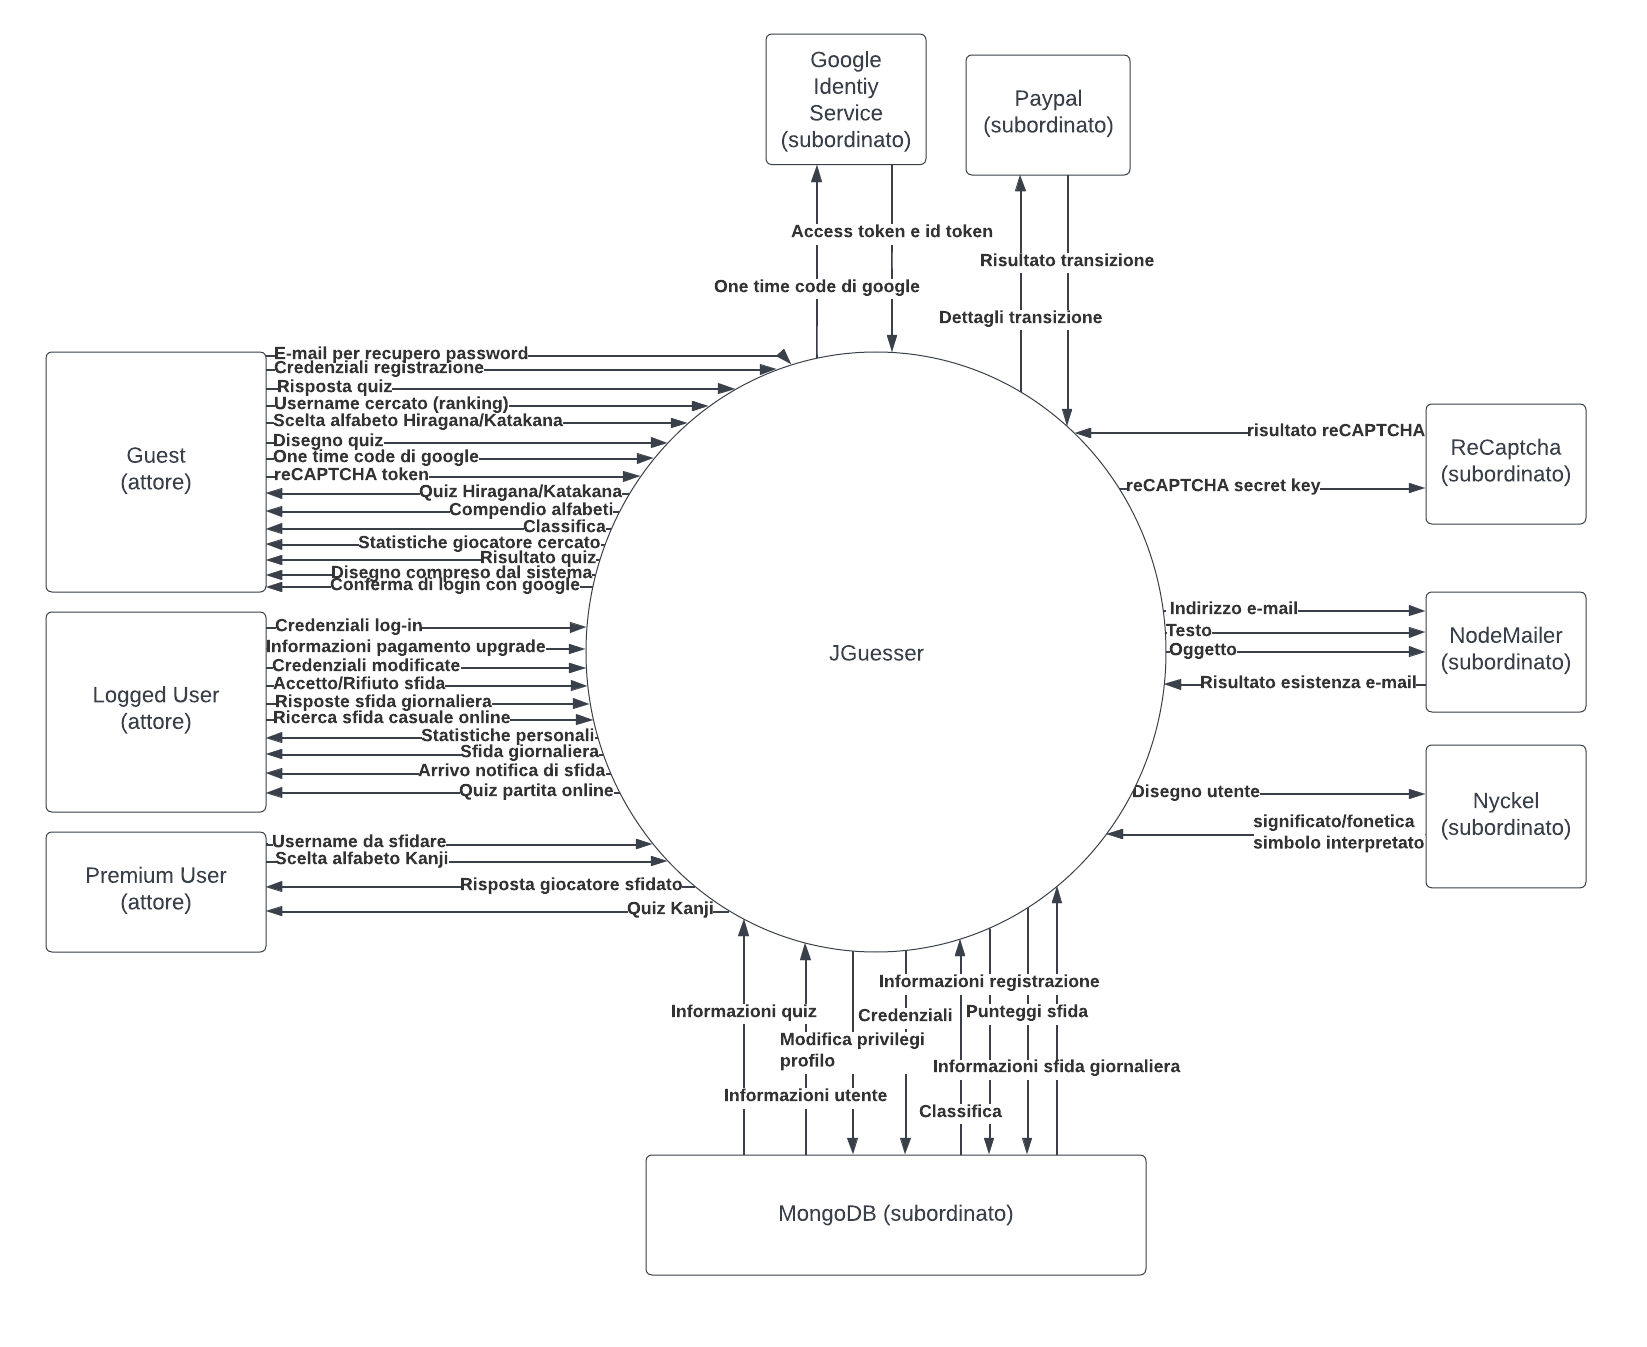
\includegraphics[scale=0.23]{images/diagramma_di_contesto.png}
\caption{Diagramma di contesto dell'applicazione JGuesser}
\label{fig:diagramma_di_contesto}
\end{figure}
\noindent

\subsection{Descrizione interazioni attori e sistemi esterni}
In questa sezione vengono descritti i diversi flussi d'informazione per ogni attore o sistema esterno.

\subsubsection{Guest}
Guest è l'attore che rappresenta l'utente che non è loggato all'interno del sistema. L'utente guest invia una serie di dati in ingresso al sistema JGuesser:
\begin{itemize}
    \item E-mail per recupero password: flusso che rappresenta l'invio di un'email di uno degli account registrati all'interno dell'applicazione JGuesser.
    \item Credenziali registrazione: flusso che rappresenta l'invio dei dati che l'utente utilizza per registrarsi (username, e-mail, password e nazione).
    \item Risposta quiz: flusso che rappresenta l'invio della risposta da parte dell'utente ad uno specifico quiz.
    \item Username cercato (ranking): flusso che rappresenta l'invio del username del giocatore che si vuole ricercare in classifica.
    \item Scelta alfabeto Hiragana/Katakana: flusso che rappresenta l'invio degli alfabeti selezionati dall'utente nel caso in cui questo abbia scelto come modalità di gioco 'training' del single-player.
    \item Disegno quiz: flusso che rappresenta l'invio dell'immagine del simbolo disegnato dall'utente nel caso in cui questo abbia giocato al quiz di tipo 4.
    \item One time code di google: flusso che rappresenta l'invio al sistema del one time code, ovvero di quel codice che l'utente guest ottiene dialogando con il sistema esterno google identity service. Viene inviato per ottenere una conferma di avvenuto login con google da parte dall'applicazione JGuesser.
    \item reCAPTCHA token: flusso che rappresenta l'invio del reCAPTCHA token, ovvero di quel token che l'utente guest ottiene dialogando con il sistema esterno reCAPTCHA. Questo dato viene inviato all'applicazione, perchè si vuole ottenere una conferma dall'applicazione che l'utente abbia cliccato effettivamente sul reCAPTCHA per verificarsi.
\end{itemize}
\noindent
e riceve in ingresso le seguenti informazioni:
\begin{itemize}
    \item Quiz Hiragana/Katakana: flusso che rappresenta la ricezione dei quiz di ogni tipologia, limitati agli alfabeti Hiragana e Katakana.  
    \item Compendio alfabeti: flusso che rappresenta la ricezione della pagina che conterrà il compendio degli alfabeti.
    \item Classifica: flusso che rappresenta la ricezione dei dati della classifica, che verranno mostrati a video all'utente.
    \item Statistiche giocatore cercato: flusso che rappresenta la ricezione dei soli dati della classifica specifichi a un solo giocatore scelto dall'utente. In questo modo l'utente potrà visualizzare soltanto i dati dell'utente che gli interessano.
    \item Risultato quiz: flusso che rappresenta la ricezione del risultato del quiz, per cui l'utente ha dato una risposta. Serve per far capire all'utente se ha risposto correttamente oppure no.
    \item Disegno compreso dal sistema: flusso che rappresenta la ricezione della fonetica/significato a cui è associato il disegno che il sistema esterno Nyckel ha interpretato. Questo flusso di dati prende in considerazione sia il risultato del quiz di tipo 4, ma anche la possibile richiesta di interpretazione da parte dell'utente.
    \item Conferma di login con google: flusso che rappresenta la ricezione di un dato che confermi all'utente che il login attraverso google è avvenuto con successo e che è stato aggiornato il proprio stato.
\end{itemize}

\subsubsection{Logged User}
Logged user è l'attore che rappresenta l'utente loggato all'interno del sistema. L'utente loggato può fare tutto quello che può fare l'utente guest e e quindi eredita tutti i suoi flussi di dati in ingresso e in uscita. All'interno del diagramma di contesto per questo attore, sono stati individuati i seguenti flussi di dati in uscita diretti verso il sistema JGuesser:
\begin{itemize}
    \item Credenziali log-in: flusso che rappresenta l'invio delle credenziali (username e password) per effettuare il login.
    \item Informazioni pagamento upgrade: flusso che rappresenta l'invio delle informazioni di pagamento. Con questo flusso si vuole far sapere al sistema che si ha intenzione di effettuare il pagamento della quota per effettuare l'upgrade del proprio profilo a premium.
    \item Credenziali modificate: flusso che rappresenta l'invio delle credenziali modificate (e-mail e password). Queste devono essere inviate quando l'utente che si trova nella propria area personale ha deciso di modificare la propria e-mail o password con una nuova.
    \item Accetto/Rifiuto sfida: flusso che rappresenta l'invio del messaggio di accetto o di rifiuto di una sfida.
    \item Risposte sfida giornaliera: flusso che rappresenta l'invio delle risposte con punteggi alle sfide giornaliere.
    \item Ricerca sfida casuale online: flusso che rappresenta l'invio del username del giocatore a cui si intende inviare l'invito di sfida.
\end{itemize}
\noindent
e i seguenti flussi di dati in ingresso:
\begin{itemize}
    \item Statistiche personali: flusso che rappresenta la ricezione di tutte le statistiche personali dell'utente.
    \item Sfida giornaliera: flusso che rappresenta la ricezione dei quiz di sfida giornaliera.
    \item Arrivo notifica di sfida: flusso che rappresenta la ricezione della notifica di sfida. La notifica viene ricevuta quando l'utente viene sfidato personalmente da un utente premium.
    \item Quiz partita online: flusso che rappresenta la ricezione del quiz di una partita online. Differisce dal Quiz Hiragana/Katakana, perchè su questo tipo di flusso possono viaggiare anche quiz di tipo Kanji, che nel single-player può scegliere soltanto il premium user. 
\end{itemize}

\subsubsection{Premium User}
Il premium user è l'attore che rappresenta l'utente che ha effettuato l'aggiornamento del proprio account a premium. Il premium user eredita tutti i flussi di dati da parte del logged user. Per il premium user sono stati identificati i seguenti flussi di dati in uscita:
\begin{itemize}
    \item Username da sfidare: flusso che rappresenta l'invio del username che il premium user vuole sfidare (multiplayer).
    \item Scelta alfabeto Kanji: flusso che rappresenta l'invio di un'informazione che dica al sistema che l'utente ha scelto l'alfabeto Kanji nella modalità 'training' del single-player.
\end{itemize}
\noindent
e i seguenti flussi di dati in ingresso:
\begin{itemize}
    \item Risposta giocatore sfidato: flusso che rappresenta la ricezione di un'informazione che dica all'utente sfidante, se questo invito è stato accettato oppure no.
    \item Quiz Kanji: flusso che rappresenta la ricezione dei quiz Kanji durante il training.
\end{itemize}

\subsubsection{Google Identity Service}
Google Identy Service è il sistema esterno che permetterà all'utente guest di effettuare l'accesso con le proprie credenziali google. Questo attore dovrà comunicare con l'applicazione JGuesser e con l'attore guest per verificare e quindi di conseguenza confermare l'accesso di un determinato utente tramite google. Nel diagramma di contesto sono stati individuati due flussi di dati. Un flusso di dati in ingresso al sistema Google Identity Service e un flusso di dati in uscita. Il flusso di dati in ingresso è rappresentato dal One time code che è un dato che l'utente avrà precedentemente inviato all'applicativo JGuesser e che il sistema dovrà inviare al sistema esterno per ricevere gli altri dati dell'utente. Ottenuti gli altri dati dell'utente, che sono l'access token e l'id token attraverso il flusso di uscita, l'applicativo potrà confermare il login con google. Questo sistema esterno compare nel RF\ref{req_login_con_google}.

\subsubsection{Paypal}
Paypal è il sistema esterno con cui l'applicativo JGuesser dovrà interfacciarsi per permettere all'utente registrato di effettuare il pagamento di 2.99\EUR{} all'indirizzo email \href{mailto:lorenzo.dambro@gmail.com}{lorenzo.dambro@gmail.com}. Per il seguente sistema sono stati individuati due flussi di dati. Un flusso di dati in ingresso e un flusso di dati in uscita. Il flusso di dati in ingresso rappresenta i dettagli della transazione che saranno forniti dall'applicazione. Il flusso di dati in uscita invece rappresenta il risultato della transazione e quindi verrà restituito al sistema JGuesser un valore, che gli permetterà di capire se la transazione è andata a buon fine oppure se ci sono stati degli errori. \\
Questo sistema compare e serve a soddisfare il RF\ref{req_profilo_premium}.

\subsubsection{reCaptcha}
ReCAPTCHA è il sistema esterno con cui l'applicazione JGuesser si dovrà interfacciare per ottenere la conferma che l'utente non è un bot. In particolare questo tipo di sistema sarà coinvolto quando l'utente dovrà registrarsi e quando l'utente vorrà resettare la propria password. Nel diagramma di contesto sono stati identificati due flussi, uno in ingresso al sistema reCAPTCHA e l'altro in uscita. Il flusso d'ingresso è rappresentato dalla chiave segreta del sito, che sarà inviata al sistema reCAPTCHA, che dovrà rispondere con una verifica di successo/fallimento del token. Questa risposta è stata rappresentata nel diagramma attraverso l'unico flusso di uscita presente. \\
Questo sistema esterno è presente nei RF\ref{req_registrazione} e RF\ref{req_recupero_nome_utente_e_password}.

\subsubsection{Nodemailer}
Nodemailer è il sistema esterno che si occuperà di inviare tutte le e-mail che l'applicativo JGuesser necessita di inviare e che verificherà ogni singola e-mail che gli utenti inseriranno. All'interno del diagramma di contesto sono stati identificati quattro flussi di dati di cui tre in ingresso, che rappresentano: 
\begin{itemize}
    \item e-mail;
    \item oggetto;
    \item testo.
\end{itemize}
\noindent
e uno in uscita che rappresenta un dato che permetterà di capire se l'e-mail fornita è un'e-mail valida e quindi effettivamente esistente oppure no. Il sistema JGuesser necessità di inviare e-mail nei seguenti 3 casi:
\begin{itemize}
    \item un utente si è registrato e quindi viene inviata un e-mail di conferma avvenuta della registrazione. Vedere RF\ref{req_registrazione}.
    \item un utente ha dimenticato le proprie credenziali e quindi deve essere inviata un e-mail con le nuove credenziali. Vedere RF\ref{req_recupero_nome_utente_e_password}.
    \item un utente ha effettuata l'upgrade del proprio profilo a premium e quindi viene inviata un e-mail di ringraziamento all'utente. Vedere RF\ref{req_profilo_premium}.
\end{itemize}

\subsubsection{Nyckel}
Nyckel è il sistema esterno che attraverso una serie di API, riuscirà a classificare i simboli dei diversi alfabeti, che l'utente andrà a disegnare. Nel diagramma di contesto sono stati specificati due flussi, uno in ingresso a Nyckel e l'altro in uscita. Quello in ingresso rappresenta il disegno che l'utente potrà disegnare nel quiz di tipo 4. Quello in uscita invece rappresenta la risposta e quindi la fonetica/significato del simbolo che Nyckel ha classificato. \\
Questo sistema esterno entra in gioco nel RF\ref{req_quiz_4}.

\subsubsection{MongoDB}
MongoDB è il sistema esterno, che verrà utilizzato all'interno dell'applicazione per memorizzare tutte le informazioni riguardanti gli utenti, sia informazioni personali che statistiche. Oltre a ciò si utilizzerà per memorizzare tutte le informazioni riguardanti i simboli dei diversi alfabeti giapponesi. Nel diagramma di contesto sono stati identificati una serie di flussi di dati in ingresso:
\begin{itemize}
    \item Informazioni registrazione: flusso che rappresenta la ricezione dal sistema delle informazioni di registrazione (username, password, nazione).
    \item Credenziali: flusso che rappresenta la ricezione delle credenziali utenti (username/email, password).
    \item Modifica privilegi profilo: flusso che rappresenta la ricezione di un dato che fa capire al database che deve aggiornare i privilegi dell'utente a premium.
    \item Punteggi sfida: flusso che rappresenta la ricezione dei punteggi di ogni singola sfida online e di ogni singola sfida giornaliera che l'utente gioca.
\end{itemize}
\noindent
e una serie di flussi di dati in uscita:
\begin{itemize}
    \item Informazioni utente: flusso che rappresenta l'invio di tutte le informazioni utente, che servono per soddisfare diversi RF.
    \item Informazioni quiz: flusso che rappresenta l'invio delle informazioni dei quiz che poi verranno inviata all'utente per visualizzare e svolgere il quiz.
    \item Classifica: flusso che rappresenta l'invio delle informazioni della classifica, che l'utente ha richiesto di visualizzare.
    \item Informazioni sfida giornaliera: flusso che rappresenta l'invio delle informazioni dei quiz giornalieri.
\end{itemize}
\noindent
Questo sistema esterno è stato utilizzato per soddisfare moltissimi requisiti funzionali, quasi tutti.